% !TeX root = ../thesis.tex

\begin{savequote}[85mm]
    I don’t want to insist on it, Dave, but I am incapable of making an error.
    \qauthor{HAL 9000}
    \end{savequote}
    
\chapter{Explore Strategies to Transform Health Data Into Actionable Decisions and Policies}\label{chap:goal3}

\initial{T}his chapter focuses on the practical application of health data in influencing decisions and policies, particularly in the realms of drug evaluation and obstetrics, as detailed in sections \ref{subsec:ipop} and \ref{subsec:obs}.

Section \ref{subsec:ipop} represents an innovative application of causality principles and transparent \ac{ml} models to assess the real-world effectiveness of two groups of breast cancer drugs. Beginning with traditional analysis methods, the study progressively adopts more complex techniques, including \ac{iptw} to enhance the comparative assessment of these treatments. This approach exemplifies how health data, analyzed through advanced methodologies, can influence drug policy and treatment choices in clinical settings.

Section \ref{subsec:obs} is an extension of research in distributed data mechanisms (referenced in section \ref{subsec:distributed}), uses \ac{ml} to develop a \ac{cdss} designed to assist in evaluating \ac{cs}. The system's interoperability and its focus on supporting subpar evaluation of \ac{cs} demonstrate the utilization of health data in creating tools that aid in decision-making processes in obstetrics. This section underscores the importance of applying health data analytics in real-time clinical environments to inform decisions and shape obstetrical policies.



\section{How Can We Leverage Data to Assess Treatment Efficacy?}\label{subsec:ipop}
This section is based on the paper entitled "Comparative Analysis of Palbociclib and Ribociclib: A real world data and Propensity Score-Adjusted Evaluation with endocrine therapy". This was a method of applying the knowledge of causality and transparent \ac{ml} models in order to assess the real-world effect of two drugs for breast cancer. We started with traditional analysis and then moved to a more complex approach, using \ac{iptw} methods in order to further compare treatments.
    
    
\subsection{Introduction}
    Currently, metastatic breast cancer is difficult to treat. Patients with \ac{hr+} and \ac{her2} breast cancer, the most common subtype, typically undergo \ac{et}. Therefore, new treatments can be very useful in improving quality of life, reducing toxicity, and decreasing scenarios of hormonal resistance.
Medications from the group of \ac{cdk46i} appear as a potential improvement in the therapeutic approach to advanced breast cancer. Within this group, there are palbociclib, ribociclib and abemaciclib. \ac{cdk46} are responsible for regulating the cell cycle at the transition between the G1 and S phases. In many neoplasms, this cycle is deregulated, and it promotes uncontrolled cell proliferation. It is then possible for these medications to have better effectiveness. These medications were approved by INFARMED, I.P. after an analysis of the therapeutic value they offer. This decision was made based on data provided by clinical trials done with these medications. The MONALEESA \cite{hortobagyiUpdatedResultsMONALEESA22018, slamonPhaseIIIRandomized2018, tripathyRibociclibEndocrineTherapy2018} studies were used for ribociclib, PALOMA \cite{vermaPalbociclibCombinationFulvestrant2016, rugoImpactPalbociclibLetrozole2018, finnCyclindependentKinaseInhibitor2015a} for palbociclib, and MONARCH \cite{goetzMONARCHAbemaciclibInitial2017, sledgeMONARCHAbemaciclibCombination2017} for abemaciclib.
These studies focused on testing the hypothesis of treating \ac{cdk46i} in combination with an aromatase inhibitor or fulvestrant as an alternative to the gold standard. In these research findings, it was determined that there was a notable enhancement in effectiveness, supporting their application in clinical practice.
However, this evaluation was based on clinical trials with very specific inclusion and exclusion criteria and in a highly controlled environment. It is then vital to study how these new molecules compare to current practice in terms of treatment effectiveness in a real-world setting. In the meticulously controlled setting of clinical trials, patient selection often skews towards relatively healthier individuals with fewer comorbidities. However, in real-world clinical practice, patients present a diverse range of health profiles, co-existing illnesses, and medication histories that may influence drug efficacy and safety. Real-world data, drawn from electronic health records, insurance claims databases, and patient registries, offers the advantage of reflecting a more heterogeneous patient population, thus potentially uncovering insights not readily apparent in clinical trial settings. Understanding the effectiveness and safety of \ac{cdk46i} in real-world conditions is crucial for tailoring more individualized treatment regimens, optimizing outcomes, and enhancing the quality of life for patients with \ac{hr+}, \ac{her2} breast cancer \cite{harbeckCDK4InhibitorsHR2021}. Nevertheless, observational studies have inherent limitations, such as confounding by indication, which can lead to biased estimates of treatment effects. To tackle this, there are causality-based assessments that can be employed in order to better estimate the causal effects of treatments.
Incorporating statistical techniques like \ac{iptw} can play an essential role in enhancing the quality of real-world evidence by accounting for treatment selection bias and balancing observed covariates between treatment groups. \ac{iptw}, grounded in the framework of causal inference, allows for the mimicking of a randomized control trial-like setting within observational studies. By assigning weights to individual patients based on their propensity scores—the likelihood of receiving a particular treatment given a set of observed characteristics—analyses can achieve a balance between different treatment arms, thereby reducing bias and confounding factors. Establishing causality, rather than mere association, is vital for the robust interpretation of real-world data. As we strive to understand the long-term impact, efficacy, and safety of \ac{cdk46i} in \ac{hr+}, \ac{her2} breast cancer, the rigorous application of \ac{iptw} and causal inference methods can substantially augment the validity of real-world findings, making them a more reliable basis for clinical decision-making \cite{austinIntroductionPropensityScore2011,austinUsePropensityScore2014}
So in this paper, we propose:
\begin{itemize}
    \item To compare the effectiveness of the \ac{cdk46i} drug class in terms of  \ac{pfs}  and \ac{os} \ac{os};

    \item To assess the Hazard Ratio of using the \ac{cdk46i} drug class in terms of \ac{pfs} and \ac{os}.
    
    \item  To compare the effectiveness of \ac{cdk46i} in combination with letrozole or fulvestrant with the previous standard of care in terms of \ac{pfs} and \ac{os} in patients with \ac{hr+}, \ac{her2} advanced breast cancer with bone only metastasis.

    \item To assess the differences in effectiveness between the three \ac{cdk46i} in combination with letrozole or fulvestrant in terms of \ac{pfs} and \ac{os} with causality principles in mind, especially the counterfactual theory and \ac{iptw}.
    
\end{itemize}

    \subsection{Materials \& Methods}
    

\subsection{Study Design}

This retrospective study was designed in 2022. The study aimed to evaluate the clinical benefit and long-term survival of patients with \ac{hr+}/\ac{her2} that started treatment with \ac{cdk46i} plus \ac{et} in different lines of treatment between the 14th of March 2017 and the 31st of December 2021. The follow-up period was set until June 2022. Inclusion criteria: women and men, \ac{hr+} and \ac{her2} in the primary tumor or metastatic site after biopsy. Exclusion criteria: Patients that had only one ambulatory medication, and patients involved in clinical trials, diagnosed with other neoplasms or with active treatment during the study period. The control group was defined by a population of patients, that were treated with hormone therapy as first-line (due to bone metastases only) between 2015 and 13 of match 2017.
The evaluation of effectiveness will involve \ac{os} and progression-free analysis. We will compare the two different \ac{cdk46i} in terms of effectiveness in real-world patients and will also compare the effectiveness of this class combined with \ac{et} against traditional \ac{et}.


\subsection{Data collection}
All data were collected from medical and administrative records from baseline to last visit or death. The data was collected from Instituto Português de Oncologia – Porto (IPO-P). Table 1 shows a comparison between the groups.
Data included for population treated with \ac{cdk46i} plus \ac{et}: demographic information, age at first diagnosis and age at the beginning of treatment, clinical characteristics and performance status by  \ac{ecog}, treatment line and treatment schema - CDK4/6 inhibitor and \ac{et}, stage of cancer, site of metastases (bone, soft tissue, visceral, central nervous system with or without another site).
Data included for the population treated with \ac{et} as first-line: demographic information, age at first diagnosis and age at the beginning of treatment, clinical characteristics and performance status by  \ac{ecog}, stage of the cancer.
For comparison purposes, we used palbociclib and ribociclib since we had a small number of patients treated with abemaciclib (12).

 
\begin{table}
\caption{Descriptive statistics of \ac{cdk46i} group and \ac{et} group. The Drug/combination refers to the actual drug or the combination for CDK4/6}
\centering
\label{tab:stats_ipop_cdk}

\begin{tabular}[t]{llll}
\toprule
  &\ac{et}& Palbociclib & Ribociclib\\
\midrule
 & (N=43) & (N=246) & (N=106)\\
\addlinespace[0.3em]
\multicolumn{4}{l}{\textbf{Age at treatment start}}\\
\hspace{1em}Mean (SD) & 60.1 (12.4) & 59.2 (11.7) & 58.2 (10.7)\\
\hspace{1em}Median [Min, Max] & 62.0 [34.0, 85.0] & 60.0 [28.0, 84.0] & 58.0 [32.0, 79.0]\\
\addlinespace[0.3em]
\multicolumn{4}{l}{\textbf{Bone Only metastases}}\\
\hspace{1em}No & NA & 161 (65\%) & 74 (70\%)\\
\hspace{1em}Yes & NA & 85 (35\%) & 32 (30\%)\\
\hspace{1em}Missing & 43 (100\%) & 0 (0\%) & 0 \vphantom{1} (0\%)\\
\addlinespace[0.3em]
\multicolumn{4}{l}{\textbf{Visceral metastasis}}\\
\hspace{1em}No & NA & 121 (49\%) & 49 (46\%)\\
\hspace{1em}Yes & NA & 125 (51\%) & 57 (54\%)\\
\hspace{1em}Missing & 43 (100\%) & 0 (0\%) & 0 (0\%)\\
\addlinespace[0.3em]
\multicolumn{4}{l}{\textbf{Stage}}\\
\hspace{1em}I & 3 (7\%) & 22 (9\%) & 7 (7\%)\\
\hspace{1em}II & 20 (47\%) & 75 (30\%) & 22 (21\%)\\
\hspace{1em}III & 11 (26\%) & 74 (30\%) & 18 (17\%)\\
\hspace{1em}IV & 2 (5\%) & 65 (26\%) & 46 (43\%)\\
\hspace{1em}Missing & 7 (16.3\%) & 10 (4.1\%) & 13 (12.3\%)\\
\addlinespace[0.3em]
\multicolumn{4}{l}{\textbf{Drug/Combination}}\\
\hspace{1em}Anastrozol & 3 (7\%) & NA & NA\\
\hspace{1em}Exemestane & 4 (9\%) & NA & NA\\
\hspace{1em}Fulvestrant & 5 (12\%) & 180 (73\%) & 10 (9\%)\\
\hspace{1em}Letrozol & 31 (72\%) & 66 (27\%) & 96 (91\%)\\
\bottomrule
\end{tabular}

\end{table}




\subsection{Statistical Analysis}
%copied
R was used for statistical analysis. Demographic, clinical characteristics and side effects were analyzed using descriptive statistics (count, percentages and median/range). Kaplan–Meier test was used to determine the median \ac{pfs} and \ac{os} in the entire population and subgroups. Log-rank test was used for comparisons of \ac{pfs} and \ac{os} among different subgroups. Cox Regression was used to assess feature importance and impact. All statistical tests were two-sided, and the significance level was 0.05. The evaluation of the proportional hazards assumptions was done by \textit{Schoenfeld} residues analysis.
We applied propensity score weights to achieve a more robust comparison between the two groups of CDK4\/6i. We used the existence of visceral metastases, treatment line, age at treatment start, and stage. We used the WeightIt package for R \cite{WeightIt}. We applied the weights to the Kaplan-Meier curves and to the Cox Regression. We applied the weights to get the \ac{ate} which is $E[Y_i(1)-Y_i(0)]$, the average effect of moving an entire population from untreated to treated, or from one drug to the other. Weights were used instead of matching since it is more suited for calculating \ac{ate} and the need to preserve the sample size since it is already small from the start. The formula for calculating the weights was through propensity score weighting with \ac{glm}. Multiple comparisons were done with the \ac{bh} method. 



%Pretende-se que \ac{os} dados venham do Instituto Português de Oncologia – Porto (IPO-P). Pretende-se utilizar a base de dados do hospital dos últimos 5 anos.
%O estudo será registado e respeitará todos \ac{os} requisitos éticos de aprovação a comissão de ética de cada instituição participante. Caso a instituição tenha um encarregado de Proteção de Dados (EPD), este será contactado a fim de dar seu parecer, e caso necessário, a sua opinião para melhorar possíveis pontos relacionados à segurança de dados.

%The goal is to identify the clinical or biological variables that have the most impact on a specific outcome. To achieve this, considering the statistical models found, we can model things in terms of time series or survival trees to group outcomes and the clusters found. With this, we can analyze the effectiveness of the clinical course, probabilities of recurrence, or survival rates by subgroup. These models and relationships can form the basis of a clinical decision support system and can be crucial for making better healthcare decisions.

%Some of the techniques used are unsupervised techniques such as k-means, DBSCAN, or hierarchical clustering.
%The goal is to identify the clinical or biological variables that have the most impact on a specific outcome. To achieve this, considering the statistical models found, we can model things in terms of time series or survival trees to group outcomes and the clusters found. With this, we can analyze the effectiveness of the clinical course, probabilities of recurrence, or survival rates by subgroup. These models and relationships can form the basis of a clinical decision support system and can be crucial for making better healthcare decisions.

%Some of the techniques used are unsupervised techniques such as k-means, DBSCAN, or hierarchical clustering.

    \subsection{Results}
    The median \ac{os} in the entire population treated with \ac{cdk46i} was 46 months (95\% CI 39.4–55.6). Median \ac{pfs} was 20.1 months (95\% CI 18.3–24.2). Following this, we compared Palbociclib and ribociclib only as first-line treatments. We found that regarding \ac{os}, there is no significant difference between the two, but ribociclib is significantly better in terms of \ac{pfs} (\textit{P} value $\le$ 0.001) (Figure \ref{fig:interest}). Additionally, we compared the same \ac{cdk46i} with letrozole as a combination only (PAL-LT and RIB-LT). Regarding this scenario, we found out that both were similar in terms of \ac{os} and \ac{pfs}.


\begin{figure}[ht]
  \caption[Survival curves for Palbociclib and Ribociclib (1st line)]{Survival curves for Palbociclib and Ribociclib (1st line) - \ac{pfs} and \ac{os}}\label{fig:interest} 
  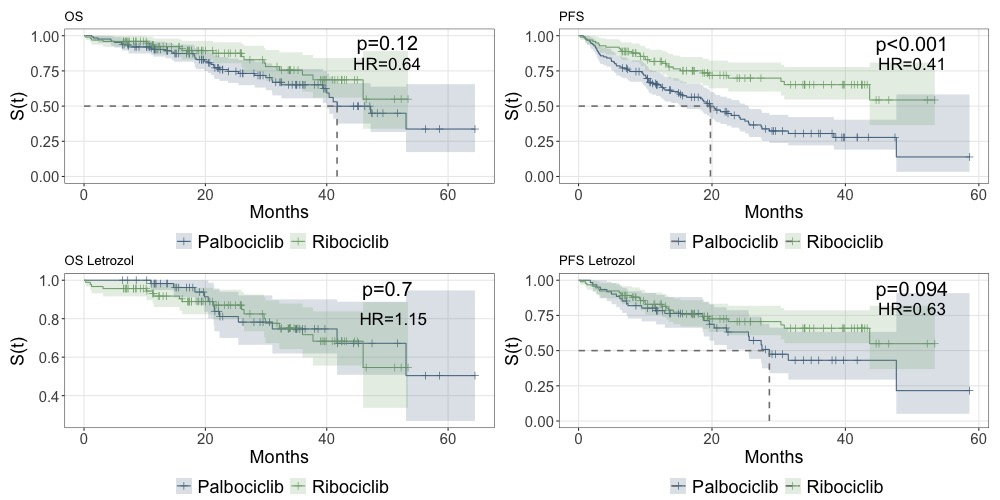
\includegraphics[scale=0.45]{figures/interest_curve_both.jpeg}%

\end{figure}


We then compared both with a cox regression, where \ac{os} shows no significant difference between palbociclib and ribociclib when adjusted to the stage, visceral metastases, age, treatment line, combination and \ac{ecog}. The proportional hazards' assumption was confirmed with \textit{P} values all over 0.10.
\begin{table}[ht]
  \centering
  \caption[Cox Regression with palbociclib and Ribociclib - \acs{pfs} and \acs{os}]{Cox Regression with palbociclib and Ribociclib - \ac{pfs} and \ac{os}}\label{tab:cox} 
  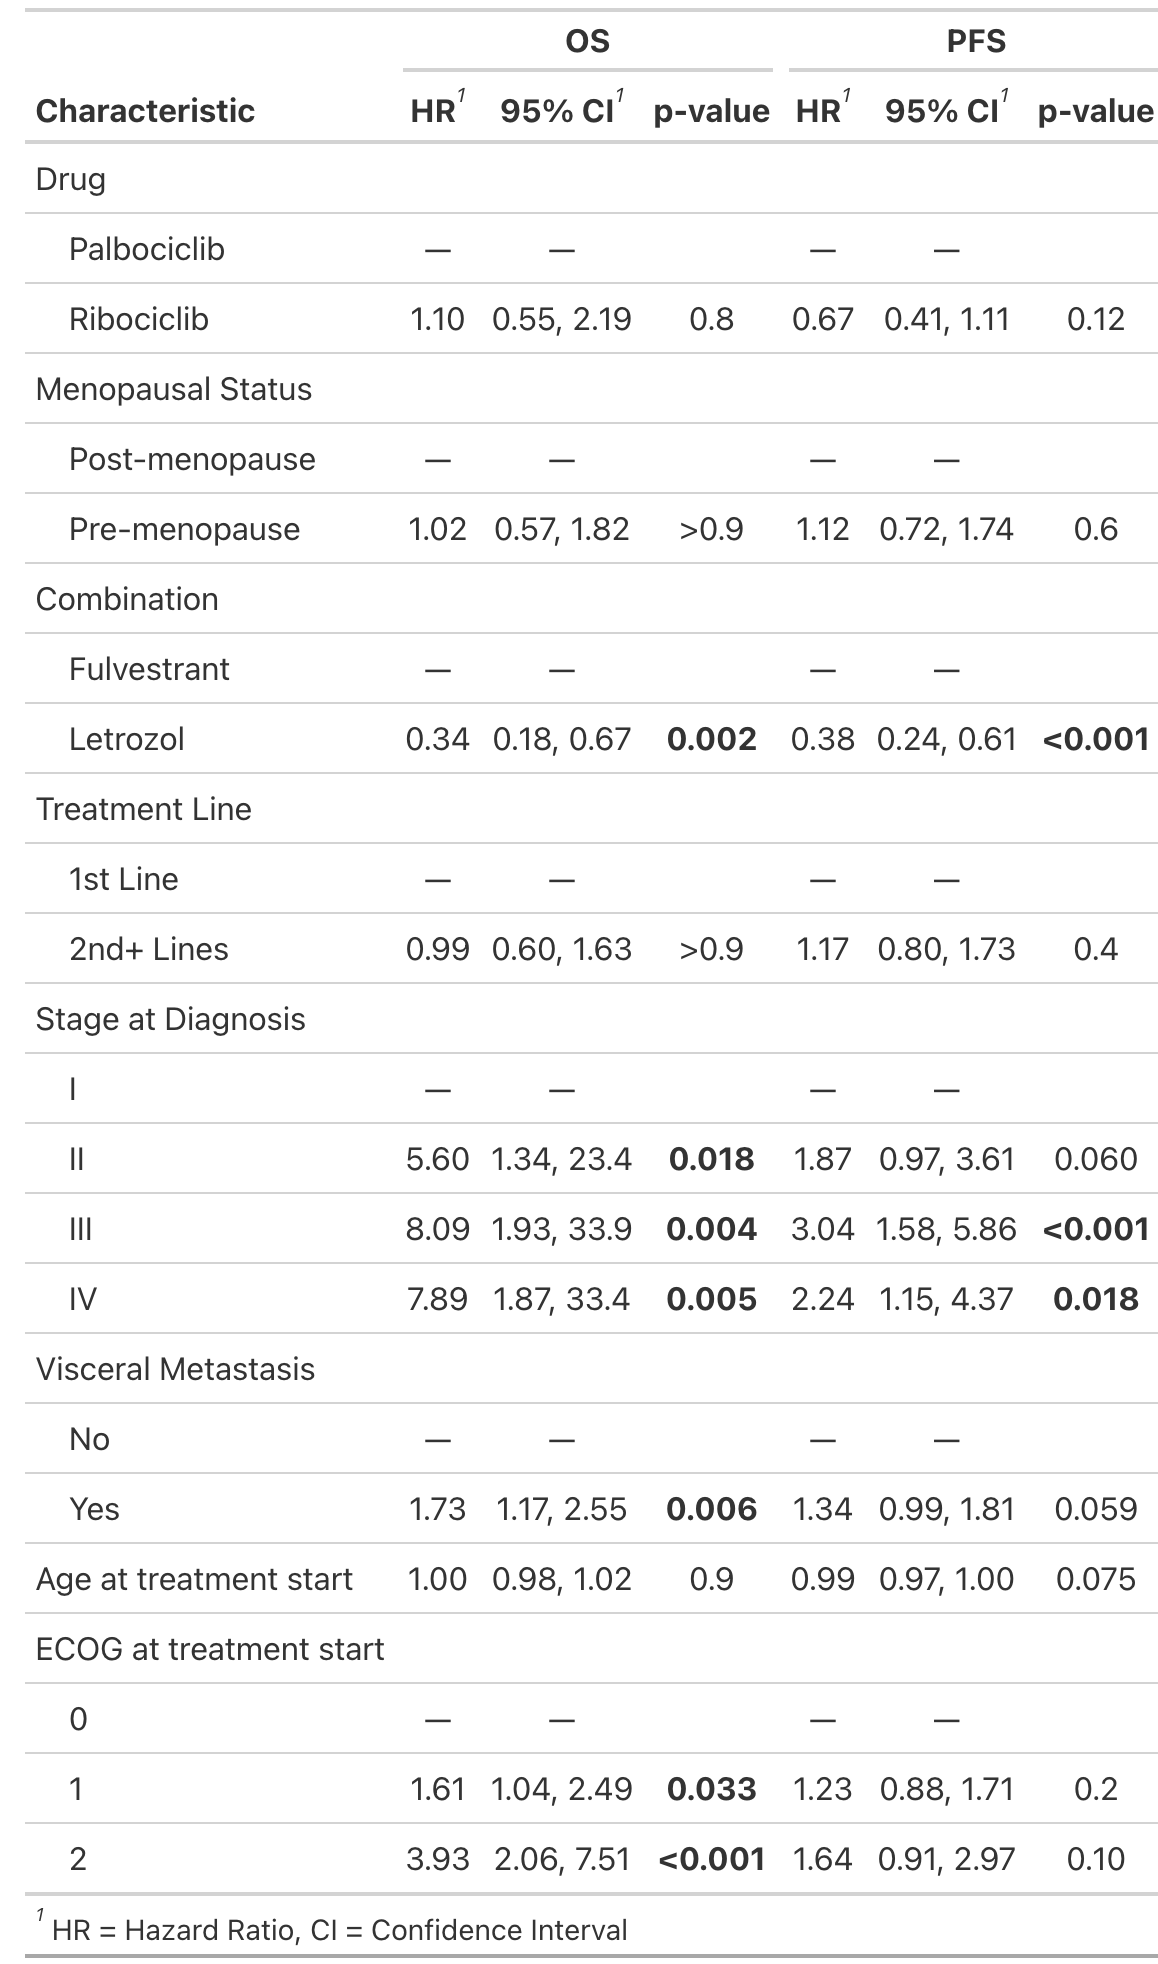
\includegraphics[scale=0.20]{figures/cox_both.png}%

\end{table}

When comparing \ac{et} with \ac{cdk46i} as first-line treatment (figure \ref{fig:grouped}). For this study we only compared patients with bone only metastasis. When comparing both \ac{cdk46i} combined with Fulvestrant or letrozole, we see that  Ribociclib (RIB+LT/FUL) is significantly better for \ac{pfs} (\textit{P} value $\le$ 0.001 \ac{hr}=0.21) but not \ac{os}. For Palbociclib as the first line with Fulvestrant or letrozole (PAL+LT/FUL), we see that there is no significant difference in terms of \ac{pfs} and \ac{os} (\textit{P}=0.57 and 0.51). We also applied the same analysis but comparing only the letrozole combination with letrozole alone (PAL-LT/RIB-LT vs LT). We found that both ribociclib and palbociclib are significantly better in terms of \ac{pfs} (\ac{hr} 0.65 for palbociclib and 0.27 for ribociclib) but not \ac{os}.
\begin{figure}[ht]
  \centering

  \caption[Survival curves (\acs{os} and \acs{pfs}) comparing \acl{et} to \acl{cdk46i} combined with fulvestrant or letrozole as 1st line.]{Survival curves (\ac{os} and \ac{pfs}) comparing \ac{et} to \ac{cdk46i} combined with fulvestrant or letrozole as 1st line. First row is \ac{cdk46i} combined fulvestrant or letrozole vs fulvestrant or letrozole. Second row is \ac{cdk46i} combined with letrozole vs letrozole alone. \textit{P} values shown as pairwise vs. ET. }\label{fig:grouped} 
  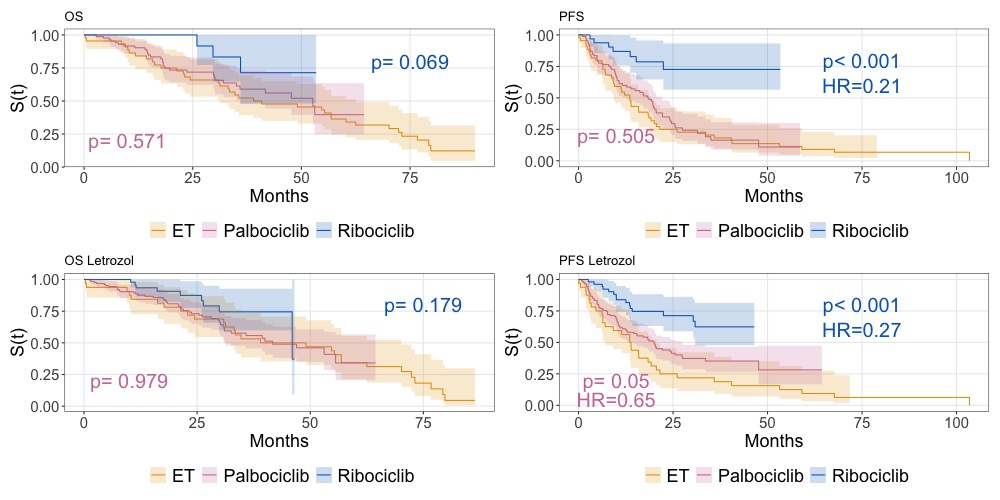
\includegraphics[scale=0.42]{figures/grouped_curve_both.jpeg}%

\end{figure}

When comparing palbociclib and ribociclib adjusted for \ac{ate} weights, we found a different scenario from previous assessments. There is a significant difference between the two in terms of \ac{os} (figure \ref{fig:propensity}). The weights were calculated as stated in the methods section.


\begin{figure}[ht]
  \centering

  \caption{Comparison of palbociclib and ribociclib survival curves adjusted for propensity scores}\label{fig:propensity} 
  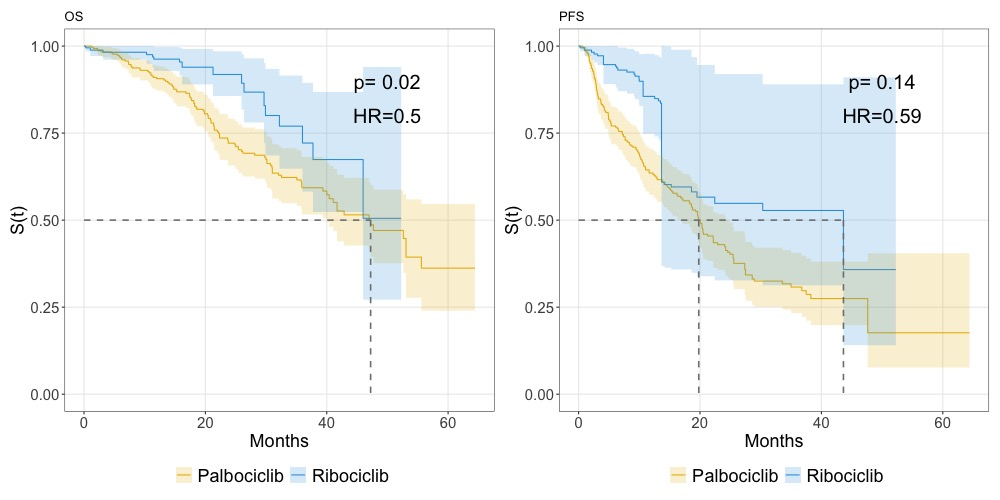
\includegraphics[scale=0.42]{figures/propensity_score_both.jpeg}%

\end{figure}

The Cox regression adjusted for the variables and with the weights applied to render an \ac{hr}=0.55 [95\% CI 0.28-1.09;\textit{P}=0.086] for \ac{os}. The \ac{hr} for \ac{pfs} is 0.56 [95\% CI 0.32-1;\textit{P}=0.05].
    \subsection{Discussion}
    The aim of this study was to evaluate the real-world use of palbociclib and ribociclib in combination with \ac{et} for \ac{hr+}/\ac{her2} and compare this drug class with traditional \ac{et}. Few real-world evidence studies of palbociclib and ribociclib used in daily clinical practice have been published identifying clinical benefit, patient profile, and sequencing of treatment, with even less evidence for the Portuguese population.

When comparing with clinical trials, regarding patient profile, in our study, 51\% had visceral metastasis and 35\% had bone-only metastases compared with 49\% and 38\% in PALOMA-2, and 60\% and 25\% in PALOMA-3, respectively \cite{rugoImpactPalbociclibLetrozole2018,cristofanilliFulvestrantPalbociclibFulvestrant2016a}.
As for ribociclib and bone-only metastases, MONALEESA-7 \cite{tripathyRibociclibEndocrineTherapy2018} has 24\% and MONALEESA-2 has 40\% \cite{hortobagyiUpdatedResultsMONALEESA22018} and our study has 30\%. Regarding menopausal status, our study has 20\% premenopausal and 80\% postmenopausal. 



Of note, the range of median \ac{pfs} for first-line palbociclib was 15.5–25.5 months, which is shorter than 27.6 months observed in a post hoc analysis of the PALOMA-2 clinical trial with extended follow-up \cite{rugoImpactPalbociclibLetrozole2018}, but in line with RWE studies (13.3–20.2 months) \cite{harbeckCDK4InhibitorsHR2021}. When assessed with only letrozole as a combination, the median \ac{pfs} increased to 28.6 months [95\% CI 25.5-not reached]. Additionally, analysing the postmenopausal women subgroup, palbociclib showed a median \ac{pfs} of 16.3 months [95\% CI 12.9 -20]. Furthering analysis of the postmenopausal and with letrozole, the median was 47.6 months [95\% 25.6-2–not reached].

As for ribociclib, median survival time was not reached whether in \ac{os} and \ac{pfs}. So we can at least say that the median \ac{pfs} is longer than 50 months. This is longer than the median \ac{pfs} of 23.8 months (95\% CI 19.2–not reached) reported in the MONALEESA-7 trial \cite{tripathyRibociclibEndocrineTherapy2018} and longer than  25.3 months (95\% CI 23.0–30.3) in the MONALEESA-2 trial \cite{hortobagyiUpdatedResultsMONALEESA22018}. Regarding the subgroup analysis of postmenopausal women, we noticed that the median was not reached for women treated with ribociclib and fulvestrant or letrozole (RIB-LT/FUL) and postmenopausal women treated with ribociclib in combination with letrozole (RIB-LT).

When directly comparing ribociclib and palbociclib without any adjustments, one might deduce that ribociclib is superior to palbociclib. However, after adjusting for confounding variables, there is no significant difference between the two inhibitors in terms of \ac{pfs} or \ac{os} as indicated in table 2. This observation is further corroborated by the lower plots in figure 1, where even a subgroup analysis of \ac{cdk46i} combined solely with letrozole reveals non-significant difference between the two.

In the first-line comparison, the analysis of \ac{os} outcomes reveals no substantial difference between \ac{et} alone and the combination of \ac{cdk46i} with \ac{et}, irrespective of whether the \ac{cdk46i} are administered with fulvestrant or letrozole  (PAL-LT/FUL vs LT/FUL; \textit{P}=0.57 | RIB-LT/FUL vs LT/FUL \textit{P}=0.069) or exclusively with letrozole (PAL-LT vs LT; p = 0.979 | RIB-LT vs LT; \textit{P}=0.179)(figure \ref{fig:grouped} left). With respect to \ac{pfs}, ribociclib demonstrates superior efficacy when compared its combination with any of the adjuvants to these adjuvants alone (RIB-LT/FUL vs LT/FUL; \ac{hr}=0.21) as well as when combined only with letrozole (RIB-LT vs LT; \ac{hr}=0.27). Additionally, palbociclib exhibits significant improvement in \ac{pfs} when combined with letrozole  (PAL-LT vs LT; \ac{hr}=0.65) (figure \ref{fig:grouped} right).
When comparing with propensity scores weighting, we found out that ribociclib is significantly better than palbociclib for \ac{pfs} and \ac{os}, providing a median \ac{os} of over 40 months and median \ac{pfs} of around 42 months. Adjusted for the weighted variables, Ribociclib is not significantly better for \ac{pfs}, but has a \textit{P} value of 0.013 for \ac{os} with an \ac{hr} of 0.48. However, the Cox regression adjusted for variables and weights are not significant, even when the \textit{P} value for \ac{pfs} is 0.05. This suggests that a more in depth analysis may be necessary.



    \subsection{Conclusion}
    In conclusion, our findings underscore the efficacy of \ac{cdk46i} in real-world settings. We can confidently affirm the impact of Ribociclib on \ac{pfs}. This assertion aligns with clinical trial outcomes and real-world data further substantiates these findings. However, we cannot do the same for \ac{os}. Our results indicate that Ribociclib combined with letrozole or fulvestrant when compared to both is not superior to these alternatives used alone. The same happens when comparing ribociclib combined with letrozole with letrozole alone. 
However, we cannot do so for Palbociclib. Palbociclib combined with fulvestrant or letrozole was not significantly better than letrozole or fulvestrant alone for \ac{pfs} nor \ac{os}. This is something interesting that we want to follow up with.
Delving deeper into the characteristics of the patient population, including safety profiles, economic implications, and quality of life metrics, would be insightful. Additionally, a thorough examination of biomarkers within the population could offer invaluable insights. Finally, extending the follow-up period would be beneficial as well. We intend to explore these facets in subsequent publications.
It’s imperative to note that our data is sourced from a singular institution, limiting the capability of generalization of our results to a broader population. Nonetheless, we posit that this study lays a foundational groundwork for future research in this domain. While our evidence is rooted in observational data, and we’ve made adjustments for known confounders, the potential for residual confounding remains. Although the use of propensity score matching enhances the comparative robustness between the groups, the presence of unmeasured confounders cannot be entirely ruled out. Furthermore, the small sample size of our study limits the statistical power of our findings. For next steps we aim to further analyse the clinical variables that have an impact on the outcome of the combination of CDK4/6 with fulvestrant or letrozole and these drugs used alone in order to infer pharmaeconomic implications and possible profiles of patient that would not benefit from this combination which would be vital for economic reasons and to apply in countries with low access to these drugs.
    
    
    \section{How Can We Leverage Data to Create Clinical Decision Support Systems?}\label{subsec:obs}
    This section is based on the paper entitled "Machine-learning in Obstetrics: FHIR-based Support System for predicting delivery type". This work was in part a result of the work in section \ref{subsec:distributed}. While testing for distributed mechanisms, we kind of felt that some evaluation metrics were inspiring to pursue this further. We built a \ac{cdss} system that is interoperable and aims to provide support for subpar evaluation of a \ac{cs}.
    
    \subsection{Introduction}
    The ability to provide care to both women and newborns during delivery is one of the most important aspects of healthcare and is often used as a metric to assess healthcare as a whole across different countries.
\acp{cs} are one of the most important aspects of delivering babies since it has a considerable impact on the mother's health and well-being. Despite this type of procedure increasing over the last few years, it is still illusive the reasons behind such events. Reports from 2016 suggest that this increment is a global phenomenon, being that from 1990 to 2014, this type of delivery almost increases by 3-fold from 6.7\% to 19.1\% \cite{betranIncreasingTrendCaesarean2016,chenNonClinicalInterventions2018}. Some of these impacts, being more prone to investigation in the last years, including the risk of infection, haemorrhage, organ injury and complications related to the use of anaesthesia or blood transfusion \cite{caesereanrisk1,caesereanrisk2}.
There is also a higher risk of complications in subsequent pregnancies like uterine rupture, abnormal placental implantation and the need for hysterectomy \cite{caesereanrisk3,caesereanrisk4}. As for the infant, \acp{cs} include the risk of respiratory problems, asthma and obesity in childhood \cite{caesereanrisk3}.
Facing this, in 2015, \ac{who} released a statement regarding \acp{cs} rates. Even when other complications could not be totally assessed, it was concluded that \ac{cs} rates higher than 10\% were not associated with a reduction in maternal or newborn mortality \cite{worldhealthorganizationhumanreproductionprogramme10april2015WHOStatementCaesarean2015}.

Since there is no evidence that this type of procedure is beneficial for women or babies when there is no clear need for it, the focus on filtering such cases is important \cite{chenNonClinicalInterventions2018}.
Moreover, particularly in Portugal, \acp{cs} are used as a way of financing healthcare institutions. This was implemented as a strategy of decreasing \acp{cs} across the country. A committee was created especially with the purpose of reducing the percentage of \acp{cs} nationally. One of the actions taken along this creation was the reduction of government funding for hospitals with rates of \acp{cs} above 25\%.
In 2020, the number of \acp{cs} in Portugal is about 36.3\%. Almost at the all-time high of 36.9\% in 2009 \cite{pordatacesarianas}.
So, lowering the proportion of \ac{cs} can provide health and financial benefits to institutions and populations alike. With this in mind, we developed a  machine-learning algorithm-based support system to assist clinical teams to detect cases of potentially unnecessary \acp{cs} for analysis. So in this paper, we propose:
\begin{myitemize}
    \item help to provide a method of bringing to the discussion of clinical staff possible less than optimal care regarding deliveries;
    \item elaborates on how clinical decision support systems can be developed using interoperability standards;
    \item understand, based on the gathered data, which are the more impacting features for predicting delivery type outcome;
    \item open a research path regarding the evaluation of this type of clinical decision support system prior to the delivery;
    \item Perform a concise economic analysis to assess the potential financial impact of implementing the proposed clinical decision support tool.

\end{myitemize}
    \subsection{Rationale and Related Work}
    Regarding the related work, several teams already tackled the potential of predicting the delivery type before birth. However, we believe that creating such a system may have a huge impact on the clinical team, patient and family regarding expectations. For such a system to be possible to enter clinical practice safely, as we hope this one does, several tests and evaluations should be done before going live.
On the other hand, we are aiming for a \textit{post-partum} analysis in order to signalise potential sub-optimal decisions so the clinical teams can evaluate the case afterwards, and hopefully, learn about what could have been done better.
Works and studies on this matter have been done before, related to second opinions in the healthcare practice regarding the decision of the \ac{cs} \cite{mandatorysecondopinion} and the implementation of clinical guidelines help as well \cite{reducingcaeresan}. We hope to provide support to help teams go in this direction.

Nevertheless, in the literature, there are works related to predicting a successful vaginal birth after a previous \ac{cs}, like the work of Lipschuetz et al., \cite{lipschuetzPredictionVaginalBirth2020} where a gradient boosting method was used to predict such event using prenatal data to do so. Grobman et al., \cite{grobman_development_2007} did similar work with a multivariable logistic regression model.
There was also the usage of different modalities of data for predicting delivery type. The work of Fergus et al. \cite{fergusClassificationCaesareanSection2017} introduces a method of predicting delivery type using the fetal heart rate signals. Similarly, the work from Saleem et al. \cite{saleemStrategyClassificationVaginal2019a} proposes a method of predicting delivery type using interactions between fetal heart rate and maternal uterine contraction.
Finally, there are also works that focus on predicting delivery mode before childbirth like the work of Ullah et al. \cite{ullah_reliable_2021} where a boosting algorithm was used in order to predict delivery mode with enriched datasets. Also the work of Gimovsky et al.  \cite{gimovskyBenchmarkingCesareanDelivery} where decision trees were introduced  to predict \acp{cs} by physician group. \\
However, as far as we know, there was no model tested (even in a controlled setting) in clinical practice, with no interoperable format of communication like Fast Healthcare Interoperability Resources (FHIR) or employed to \textit{post-partum} setting and finally, none with real-world data related with Portuguese hospital, making that our paper could be a novelty under very different dimensions.


%---predict c-section


    \subsection{Methods}

    \subsubsection{Clinical Comparison}
The clinical comparison was performed by sending questionnaires to clinicians with a relationship with obstetrics in order to assess 10 patients, with only access to the variables used by the model and to answer three questions for each. The first was to give a score from 1-10 of how likely that patient would give birth through C-section, then to select the feature/variable that most influenced the decision and which feature they would require to make a better assessment. We sent the questionnaire to 20 people and obtained 6 answers, totaling 60 patient assessments. For these 10 patients, we also predicted the delivery type using our model in order to compare it with the clinicians’ answers. These patients were new and were not seen by the model during the training phase.

\subsubsection{Analysis}

%We wrote all of the code in Python 3.9.7 with the usage of the \textit{scikit-learn} library \cite{scikit-learn}. All null representations were standardized. Data was prepossessed with the removal of features with high missing rates ($>$ 90\% overall). All missing value representations were standardized. The imputation process was done using the \ac{knn} imputation method (for continuous variables) or a new category (NULLIMP) for categorical variables. 
%For this purpose, the Birth Type was reduced to binary. All assisted birth were merged into vaginal birth and \ac{cs} remained as the other class. Procedures and diagnosis were also used and were encoded as binary features, we took the time to analyse each one of them in order to avoid leakage since there were procedures obviously related to \acp{cs} and vaginal deliveries.
%Feature creation was done through the free-text variable relating to the medication prescribed. Features were collected from it and converted into \ac{atc} Classification Group level 4, which stands for chemical subgroups. We also created some new features from data in the dataset, namely new categories related to the labour and condition of the baby.
%Also, a few data quality issues were addressed, like impossible values that were transformed into null. In this category, the main issues were \ac{bmi}/Weight and gestational age.
%Finally, only a few columns were selected. We used a mixture of surveying the literature and the feature with greater correlation with the outcome.
%The models tested were Logistic Regression, Decision Tree, Random Forest, 3 different Boosting methods (as implemented by \ac{xgboost}, \ac{lightgbm} and \textit{scikit-learn}) and a linear model based on Stochastic Gradient Descent.
%The evaluation was done with repeated stratified cross-validation with 10 splits and 2 repetitions.   
%The API for serving the prediction model was developed with FastAPI.

%Finally, a clinical evaluation was carried out with questionnaires sent to several obstetrics specialists in order to assess the validity and possible impact of the model.



We obtained full approval from the ethics committee before commencing the study, as detailed in the 'Ethics Approval and Consent to Participate' subsection. The need for informed consent was waived by the ethics committee. All null representations were standardized. Data were prepossessed by removing features with high missing rates (>90\% overall). The imputation process was performed using the KNN imputation method (for continuous variables) or a new category (NULLIMP) for categorical variables. Weight was categorized into percentiles defined specifically for Portuguese babies \cite{sousa-santosDevelopmentBirthweightStandard2016}. For the purpose of this study, the Birth Type was reduced to binary. All assisted birth were merged into vaginal birth and C-Section remained as the other class. Procedures and diagnoses were also used and were encoded as binary features, and we took the time to analyze each one of them in order to avoid leakage because there were procedures obviously related to C-sections and vaginal deliveries. Feature creation was performed through the free-text variable related to the prescribed medication. Medicine names were collected from it and converted into Anatomical Therapeutic Chemical (ATC) Classification Group level 4, which represents chemical subgroups. We also created some new features from data in the dataset, namely new categories related to the labor and condition of the baby. In addition, data quality issues were addressed, such as impossible values that were transformed into null values. The main variables affected by data quality were BMI/Weight and gestational age. The data were split into training and test sets in a 0.75:0.25 manner. From the overall datasets which comprised over 200 columns, only a few columns were selected (please see table \ref{tab:delivery_methods} in the results section). We used a mixture of features selected by surveying the literature \cite{irwindaMaternalFetalCharacteristics2021,deramonfernandezPredictionModeDelivery2022,parveenAnalysisCesareanSections2021} and features with a high correlation with the outcome. The tested models were Logistic Regression, Decision Tree, Random Forest, three different Boosting methods (as implemented by XGBoost, LightGBM and scikit learn) and a linear model based on Stochastic Gradient Descent. The evaluation was performed with repeated stratified cross-validation with 10 splits and 2 repetitions, with two full cycles of dividing the training set into 10 equal parts and using 9 as the training set and 1 as the validation set. This rendered table 3. The API for serving the prediction model was developed using FastAPI. We wrote all the code in Python 3.9.7.
    \subsection{Results}
    \subsubsection{The model}
The results are mainly the model that predicts the occurrence of a \ac{cs} or natural delivery. 
The evaluation metrics are present in the table below for the best hyper-parameters found for the training data.

\begin{table}[htbp]
  \centering
  \caption[Performance Metrics in the training set]{Performance Metrics in the training set with mean \ac{auroc} and 95\% \acl{ci}}
  \label{tab:performance_metrics_auc}
  \renewcommand{\arraystretch}{1.5} % Adjust the vertical spacing
  \setlength{\tabcolsep}{12pt} % Adjust the horizontal spacing
  \begin{tabular}{lcc}
    \hline
    \textbf{Metric} & \textbf{AUC} & \textbf{CI 95\%} \\
    \hline
    \ac{xgboost} & 0.8809 & 0.8799, 0.882 \\  
    Decision Tree & 0.8337 & 0.8324, 0.8349 \\
    Logistic Regression & 0.8716 & 0.8706, 0.8726 \\
    AdaBoost & 0.8753 & 0.874, 0.8766 \\ 
    \ac{lightgbm} & 0.8805 & 0.8793, 0.8817 \\ 
    Stochastic Gradient Descent & 0.8704 & 0.8694, 0.8713 \\ 
    Random Forest & 0.8752 & 0.8743, 0.8762 \\  
    \hline
  \end{tabular}
\end{table}



\ac{xgboost} and \ac{lightgbm} were the best-performing algorithms. However, we selected \ac{lightgbm} \cite{lightgbm}. since it is faster and requires less memory. The threshold selected for deploying the model was 0.7457247885715557 which rendered the metrics in the test set like it is shown in table \ref{tab:performance_metrics_threshold}.

\begin{table}[htbp]
  \centering
  \caption{Performance Metrics in the test set with chosen threshold}
  \label{tab:performance_metrics_threshold}
  \renewcommand{\arraystretch}{1.5} % Adjust the vertical spacing
  \setlength{\tabcolsep}{12pt} % Adjust the horizontal spacing
  \begin{tabular}{lc}
    \hline
    \textbf{Metric} & \textbf{Value} \\
    \hline
    Accuracy & 0.8052 \\
    Sensitivity & 0.8223 \\
    Precision & 0.9023 \\
    F1 Score & 0.8605 \\
    \hline
  \end{tabular}
\end{table}




\subsubsection{Deployment}
The purpose of this model is to be served as an \ac{api} for usage within a healthcare institution and act as a supplementary management decision support tool for obstetrics teams. And for that to happen, a health information system must make the requests to the API. Even though a concrete, vendor-specific information model and input health information system were used, we hope to create a more interoperable clinical decision support system which can be used by every system that acts upon births and obstetrics departments. That is why we built it around the \ac{hl7} \ac{fhir} standard (R5 version) in order to simplify the method of interacting with the API. This decision, opposed as to using a proprietary model for the data, sits upon the usage of \ac{fhir} resources: Bundle and Observation for request and returning the result as a message through a custom operation called "\$predict". It is intended to publish the profiles of these objects in order to facilitate access to the API using standardized mechanisms and data models - current build of the profiles \url{https://joofio.github.io/obs-cdss-fhir/}. The current spec is detailed in the following link. The process is identified in figure \ref{fig:deploy}.
We deployed this model in production in a single hospital and without a user interface, only collecting the data and prediction for later discussion and analysis. We collected 3231 requests. During this time, the number of alarms that were triggered was 123 (3.8\%). From this, we tried to understand the level of certainty for the decision and check the difference from the threshold of these alarms. The distance to the threshold for 73 was lower than 0.1 and was bigger than 0.1 for 50 (1.55\%) cases.
%TC:ignore

\begin{figure}[htbp]
\centering
\captionsetup{justification=centering}
\caption{Deployment and decision mechanism of the model}\label{fig:deploy} 
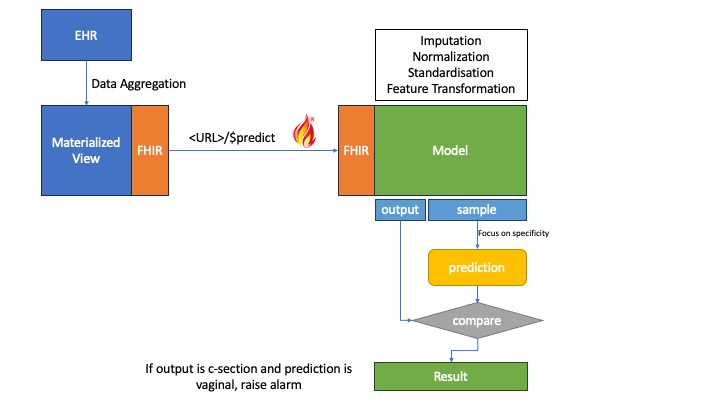
\includegraphics[scale=0.60]{figures/obs-model.jpg}
\end{figure}
%TC:endignore

\subsubsection{Clinical Evaluation}
The clinical evaluation was done by sending questionnaires to clinicians with a relationship with obstetrics in order to assess 10 patients, with only access to the variables used by the model and to answer 3 questions for each. The first was to give a score from 1-10 of how likely that patient would give birth through \ac{cs}, then to select the feature/variable that most influenced the decision and which feature they would require to make a better assessment. We sent the questionnaire to 20 people and got 6 answers. This rendered the results in figure \ref{fig:clinical}. We also predicted the result with the model as stated in figure \ref{fig:clinical}. These patients were new and not seen ever by the model in the training phase. 
As for the analysis of the most important features and missing features, the missing features were categorized into 3 categories: 1) Existent in the dataset but not included in the model, 2) Non-existent in the dataset and 3) existent in the dataset and included but that particular information was not filled for the patient assessed. This rendered a total of 62\% non-existent and 38\% existent but no information was provided at that moment. No feature mentioned existed but had not been included in the model. From the non-existent, 38\% were new clinical assessments, 38\% were linked to information from previous births,  15\% connected in more in-depth information about provided information (i.e, motive for induction) and 11\% were related to the mother's choice (if she wanted a \ac{cs}).
As for feature importance, from the 60 answers, we got 55\% with labour being the most important factor. 15\% answered the number of previous vaginal births, 8\% the evolution of weight and another 8\% the number of previous \acp{cs}. The remaining 14\% were various features, from \ac{bmi}, neuroaxis techniques, gestational age and weight of the mother. Of all of these, 90\% were included and were in the top 10 features of the model.



%TC:ignore

\begin{figure}[htbp]
\centering
\captionsetup{justification=centering}
\caption[Obstetrics questionnaires data]{Validation data. The colour represents the actual birth type. The boxplot represents the median and \ac{iqr} of the reviewers and the X represent each patient case. Contains 6 Vaginal births and 4 \acp{cs}. * represents wrong predictions of the model.}\label{fig:clinical} 
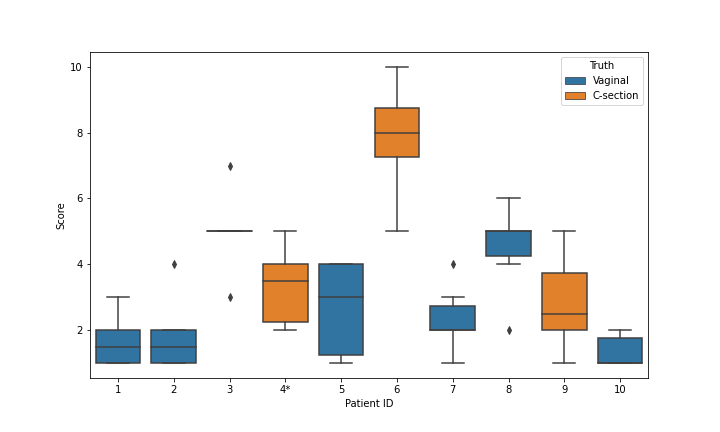
\includegraphics[scale=0.60]{figures/clinical_assessment.png}
\end{figure}
%TC:endignore


%TC:ignore

%\begin{figure}[htbp]
%\centering
%\captionsetup{justification=centering}
%\caption{Feature Importance of the model.}\label{fig:features} %
%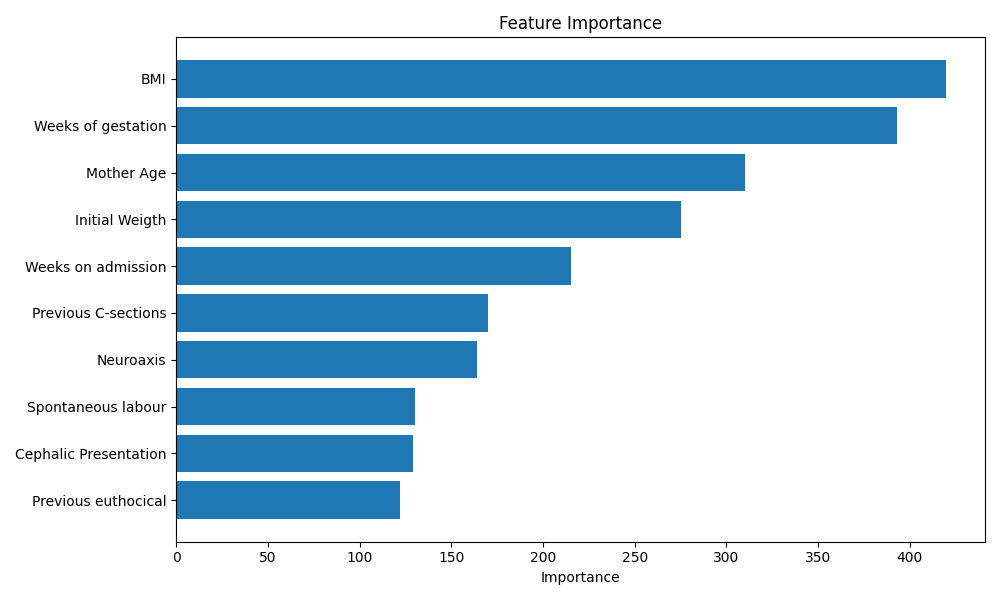
\includegraphics[scale=0.50]{figures/features.png}
%\end{figure}
%TC:endignore

\subsubsection{Potential Financial Impact}
The financial support provided to public hospitals in Portugal is partially tied to the rate of \acp{cs}. To assess the potential impact of this mechanism on all Portuguese public hospitals, we conducted a simulation study. We got data for every public hospital for the last 12 months \cite{pordatacesarianas} and applied a reduction of 3.8\% (the rate of warnings triggered in the new dataset) and recalculated the rate of \acp{cs}. The increase in support was calculated by the state-mandated rate as shown in table \ref{tab:corrections}. With this new rate, we observed that implementing our tool would result in financial benefits for 30\% (11 hospitals) of the public hospitals. Specifically, five hospitals would begin receiving support instead of no support at all. Three hospitals would experience a doubling of their financial benefit, while two hospitals would see a 50\% increase. Furthermore, one hospital would receive an additional one-third of financial support.
If we assumed that only half of the warnings found in the new data were actually true (1.9\%) we found that only 6 hospitals would be benefited. 3 from 0 to 0.25, 2 from 0.25 to 0.50 and 1 from 0.50 to 0.75.


\begin{table}[htbp]
  \centering
  \caption[Ruleset for financial support indexed to \acsp{cs}.]{Ruleset for state-provided financial support indexed to \acp{cs}. X is the current payment of a \ac{cs} inpatient episode. Adapted from \cite{acssTermosReferenciaPara2023}}
  \label{tab:corrections}
  \renewcommand{\arraystretch}{1.2} % Adjust the vertical spacing
  \setlength{\tabcolsep}{12pt} % Adjust the horizontal spacing
  \begin{tabular}{lc}
      \hline
Rate of \acp{cs}   & Support \\
    \hline
\textless 25\%       & x       \\
{[}25\%, 26.4\%{]}   & 0.75 x   \\
{[}26.5\%, 27.9\%{]} & 0.5 x    \\
{[}28\%, 29.4\%{]}   & 0.25 x   \\
\textgreater{}29,5\% & 0      \\
    \hline
\end{tabular}
\end{table}
    \subsection{Discussion}
    % !TeX root = ../../thesis.tex

The first thing to address about this model is the number of biases that we introduced in the model by choice. We joined all vaginal delivery types into a single category (assisted and non-assisted) which introduces a bias since these delivery modes are indeed different. Secondly, the fact that we want to predict if the delivery type was wrongly chosen, mainly for the case of a C-section that did not need to be so, is also a bias. We used this approach because the initially collected data did not have the representation of such events. So the biases of possibly wrong delivery types were present in the training data. We attempted to minimize this issue by selecting a threshold that gave the model higher sensitivity than specificity so that only large probabilities would trigger an alarm for human consideration. Parallel to this, we are starting to gather labelled cases, with the help of clinicians in order to create a better training dataset. Furthermore, since the data was collected from different hospitals, differences in the data input can also occur. Even though the health information system is the same, the processes that originate the data and are being used for secondary purposes could introduce several biases in the data. This is an issue that was accepted from the start regarding the mechanism of data collection and model training. Despite this, we reached a model with a very high \ac{auroc} (~88\%, 95\%CI [0.8795, 0.8815]), which is encouraging and versus the state of the art. Moreover, assuming that more data is provided and proper labelling is done regarding the outcome variable (like a clinical evaluation of needless C-sections) is added as well, a better model could be developed. Regarding the preliminary clinical evaluation, it was only possible to get an overview of the possible comparison due to the number of responders. Despite that, the results are encouraging, since the model seems to behave better than humans with the data provided. However, this is a biased vision, since clinicians in the real world have access to more data and information than the model has. It is encouraging, but caution is advised before more tests and evaluations are done. As for the deployment, future work could be the improvement of the \ac{api} in order to map all variables to an ontology like SNOMED CT or similar, making it easier for every system and person to access it and get a suggestion of the delivery type. Finally, we believe the assessment can be improved. A more robust clinical assessment is necessary as well as a thorough analysis of the impact of the tool in the real world, since we need to create the bridge between the results of the model and how clinical decisions are affected by it. A full cost-effectiveness analysis is also necessary to understand the real world impact of the model. One interesting result is the fact that 38\% of the answers regarding the most important data element missing from the patient record refers to data that is being collected but was missing for that specific patient, raising an important question about data input methodology, interoperability and quality. If we cannot have access to data when it matters most, it can become meaningless. Missing data is a problem of biomedical data as a whole. However, when specifically targeted at \ac{ml} usage of this data for predicting something, we did not find any works comparing them with clinicians. However, we did find reportsof similar missing values in obstetrics data \cite{venkateshMachineLearningStatistical2020} and we also found works of similar nature using \ac{ml} models with a robust handling of missing data such as \ac{xgboost} \cite{bitarMachineLearningAlgorithm2023} to counter this problem. This indicates that our model has the potential to counter the missing data problem as well since \ac{lightgbm} can also handle missing data natively.

    \subsection{Conclusion}
    We believe we have developed a robust system capable of detecting potentially incorrect C-section decisions, which could positively impact real-world medical practice. However, before implementation, several challenges must be addressed, particularly the need for further evaluation of the system's impact on clinical decision-making and the reasons underlying sub-optimal delivery type decisions. C-sections may be performed for various reasons, from a mother's preference to a decision made by the obstetrics team. This system is not designed to impede medical practice or to highlight flawed decisions, potentially scrutinizing specific professionals. Such caution is necessary when implementing systems like these. While having a high AUROC is beneficial, the real-world impact is another consideration. The assumptions and biases associated with autonomous systems supporting clinical practice must be carefully considered. Nonetheless, the metrics and results we have achieved so far are promising for positively influencing health and economic outcomes.
    
    
    
    